\documentclass[12pt,a4paper]{report}
\usepackage{amsmath}
\usepackage{amsfonts}
\usepackage{amssymb}
\usepackage[english]{babel} %type ngerman if you are using a PC of the university
\usepackage{babelbib}
\usepackage[T1]{fontenc}
\usepackage[utf8]{inputenc}
\usepackage{graphicx}
\usepackage[width=150mm,top=25mm,bottom=25mm]{geometry}
%\usepackage{units}
\usepackage{fancyhdr}
\pagestyle{fancy}

\renewcommand{\chaptermark}[1]{\markboth{#1}{}}

%Chapter title on even header and section title in odd header
\fancyhf{} % clear the headers
\fancyhead[R]{%
   % We want italics
   \itshape
   % The chapter number only if it's greater than 0
   \ifnum\value{chapter}>0 \chaptername\ \thechapter. \fi
   % The chapter title
   \leftmark}
\fancyfoot[C]{\thepage}

\fancypagestyle{plain}{
  \renewcommand{\headrulewidth}{0pt}
  \fancyhf{}
  \fancyfoot[C]{\thepage}
}

\setlength{\headheight}{14.5pt}
\makeatletter
\setlength{\@fptop}{0pt}
\makeatother
%\usepackage{kantlipsum} % for the mock text
\usepackage{enumerate} % enumerados
\usepackage{float} % here for H placement parameter
\usepackage{colortbl}
\usepackage{xcolor}
\definecolor{mygray}{gray}{0.8}
\usepackage{xfrac}
\usepackage{color}   %May be necessary if you want to color links
\usepackage{hyperref}
\usepackage{setspace}
\usepackage{caption}
\usepackage{subcaption}
\usepackage{titlesec}
\usepackage{tikz}
\usetikzlibrary{calc,positioning,shadows.blur,decorations.pathreplacing}
\usepackage{etoolbox}
\usepackage{anyfontsize}

%\titleformat{\chapter}{\normalfont\bfseries}{\thechapter}{1em}{\Huge}
\titleformat{\chapter}{\normalfont\bfseries}{\huge\thechapter}{1em}{\Huge}
\usepackage{nicefrac}
\onehalfspacing
\hypersetup{
    colorlinks=false, %set true if you want colored links
    linktoc=all,     %set to all if you want both sections and subsections linked
    linkcolor=blue,  %choose some color if you want links to stand out
	}
\author{Youssef El Mard Bouziani}
\title{Transversalimpulsverteilung geladener Teilchen in Proton-Proton-Kollisionen bei  $\sqrt{s} = 5.02$ TeV in ALICE}
\parindent 0ex



\begin{document}
%NEW COMMANDS
%https://texample.net/media/tikz/examples/PDF/periodic-table-of-chemical-elements.pdf
\newcommand{\Quark}[5]
{
  \begin{minipage}{0.cm}
    %\centering
      %{\scriptsize \text{#1}  \hfill  \footnotesize #2}%
      {\hfill \footnotesize \text{ #3} }
        % {\centering \footnotesize \textbf{#5}\\}
  \end{minipage}
 {\raisebox{40pt}{\makebox[1em][l]{\footnotesize \textbf{#1}}}%
 \hspace{2.3cm} \raisebox{40pt}{\makebox[3em][l]{\footnotesize \textbf{#2} }} \hspace{-3.1cm} 
       \parbox[t][1em]{3em}{\centering{\fontsize{40}{40}\selectfont  #4}	}\hspace*{1em} 
    \parbox[c][6em]{0em}{\vspace{1.4cm}\hspace{-2.7cm}\centering \footnotesize \textbf{#5}}   
}
}
  \tikzstyle{QuarkFill} = [fill=blue!15]
  \tikzstyle{LeptonFill} = [fill=red!15]
  \tikzstyle{BosonFill} = [fill=green!15]
  \tikzstyle{quark} = [draw=blue, very thick, rounded corners=2mm, QuarkFill,  minimum height={2.6cm+2pt}, minimum width=2.cm, node distance=2.cm ]
    \tikzstyle{lepton} = [draw=red, very thick, rounded corners=2mm, LeptonFill,  minimum height={2.6cm+2pt}, minimum width=1.5cm, node distance=2.cm ]
    \tikzstyle{boson} = [draw=green, very thick, rounded corners=2mm, BosonFill,  minimum height={2.6cm+2pt}, minimum width=1.5cm, node distance=2.cm ]
   
\newcommand{\pt}{$p_\text{T}$ }
    


\begin{titlepage}
\begin{center}

\vspace*{4cm}  

\huge{\textbf{Transverse momentum distributions of charged particles}}\\[2cm]
\vfill
\Large{\textbf{Bachelorarbeit}}\\
am Institut für Kernphysik Frankfurt\\
\vfill
vorgelegt von\\[1cm]
\Large{\textbf{Youssef El Mard Bouziani}}\\[1cm]
\vfill
Fachbereich Physik\\
der Goethe-Universität\\
Frankfurt am Main\\
\vspace*{1cm}
Februar 2019
\end{center}
\end{titlepage}

\vspace*{22cm}
\large{Erstgutachter: Prof. Dr. Henner Büsching}\\
\large{Zweitgutachter: Prof. Dr. Harald Appelshäuser}
\normalsize
\pagenumbering{roman}
\newpage
\tableofcontents
\newpage

\pagenumbering{arabic}
\setcounter{chapter}{-1}
\pagenumbering{arabic} 
\chapter{Abstract}

\chapter{Introduction}
%Show results in the first chapter of the thesis to have a motivation for your thesis
\label{cha:StdModel}
\section{The Structure of Matter}
\label{sec:DasSMT}
\section{Quantum Chromodynamics}
\section{Phase diagramm and Quark-Gluon-Plasma}
\section{Physics of particle collisions (pp, A-A col.)}
\begin{itemize}
\item Creation of QGP in heavy ion collisions
\item Mechanisms of the particle production (event types, elementary cross section)
\end{itemize}
\section{(charged particle) \pt spectra and nuclear modification factor}
\begin{itemize}
\item Problem statement (analysis of primary charged-particle)
\item Definition of a \pt spectrum/differential cross section (Eq. 1.19 in mknichel and also invariant yield) .
\item Definition of the nuclear modification factor and of related variables ($N_\text{coll}$, $T_\text{AA}$)
\item Present previous results of nuclear modification factors published by the charged-particle group
\end{itemize}
\section{Monte Carlo simulations}
Definition and comparison of spectra with HIJING models

\chapter{The ALICE Experiment at CERN} 
\section{The LHC}
\section{ALICE}
\subsection{ITS}
\subsection{TPC}
\subsection{Track reconstruction}
Track reconstruction (introduce the observables associated with track cuts, for example number of clusters, CHi2 per cluster, etc.), existence of a \pt resolution, introdue DCA, definition of primary particles (and secondaries)
\subsection{V0 detectors}
\subsubsection{Centrality determination}
specific for ALICE, Gabriels thesis

\chapter{Analysis}
Short introduction.
\section{Data sample}
\begin{itemize}
\item Compare data sets used for the published results with data sets (data and MC, pp and Pb-Pb) selected for this thesis. More statistics in pp allow an improved precision of \pt spectra at high \pt
\item Introduce FAST and CENT (wSDD and woSDD) reconstructions for the case of pp. Problem statement: Are FAST and woSDD similar enough to combine them?  The question will be answered later on by analysing the ratio between the corrected \pt spectra that result from CENT woSDD and CENT wSDD.
\end{itemize}
\section{Event selection}
\begin{itemize}
\item Trigger overview (working principle of the ALICE trigger), Minimum Bias
\item Selection of events in stages (selection of col. candidates, background and pile-up discrimination)
\item Introduce $|V_Z| < 10$ cm cut motivated by acceptance coverage of tracking system
\end{itemize}
\section{Track selection}
\begin{itemize}
\item Kinematik propierties.  \pt and $\eta$ range. Present track cuts.
\end{itemize}
\section{Corrections}
\begin{figure}[tb!]
\centering
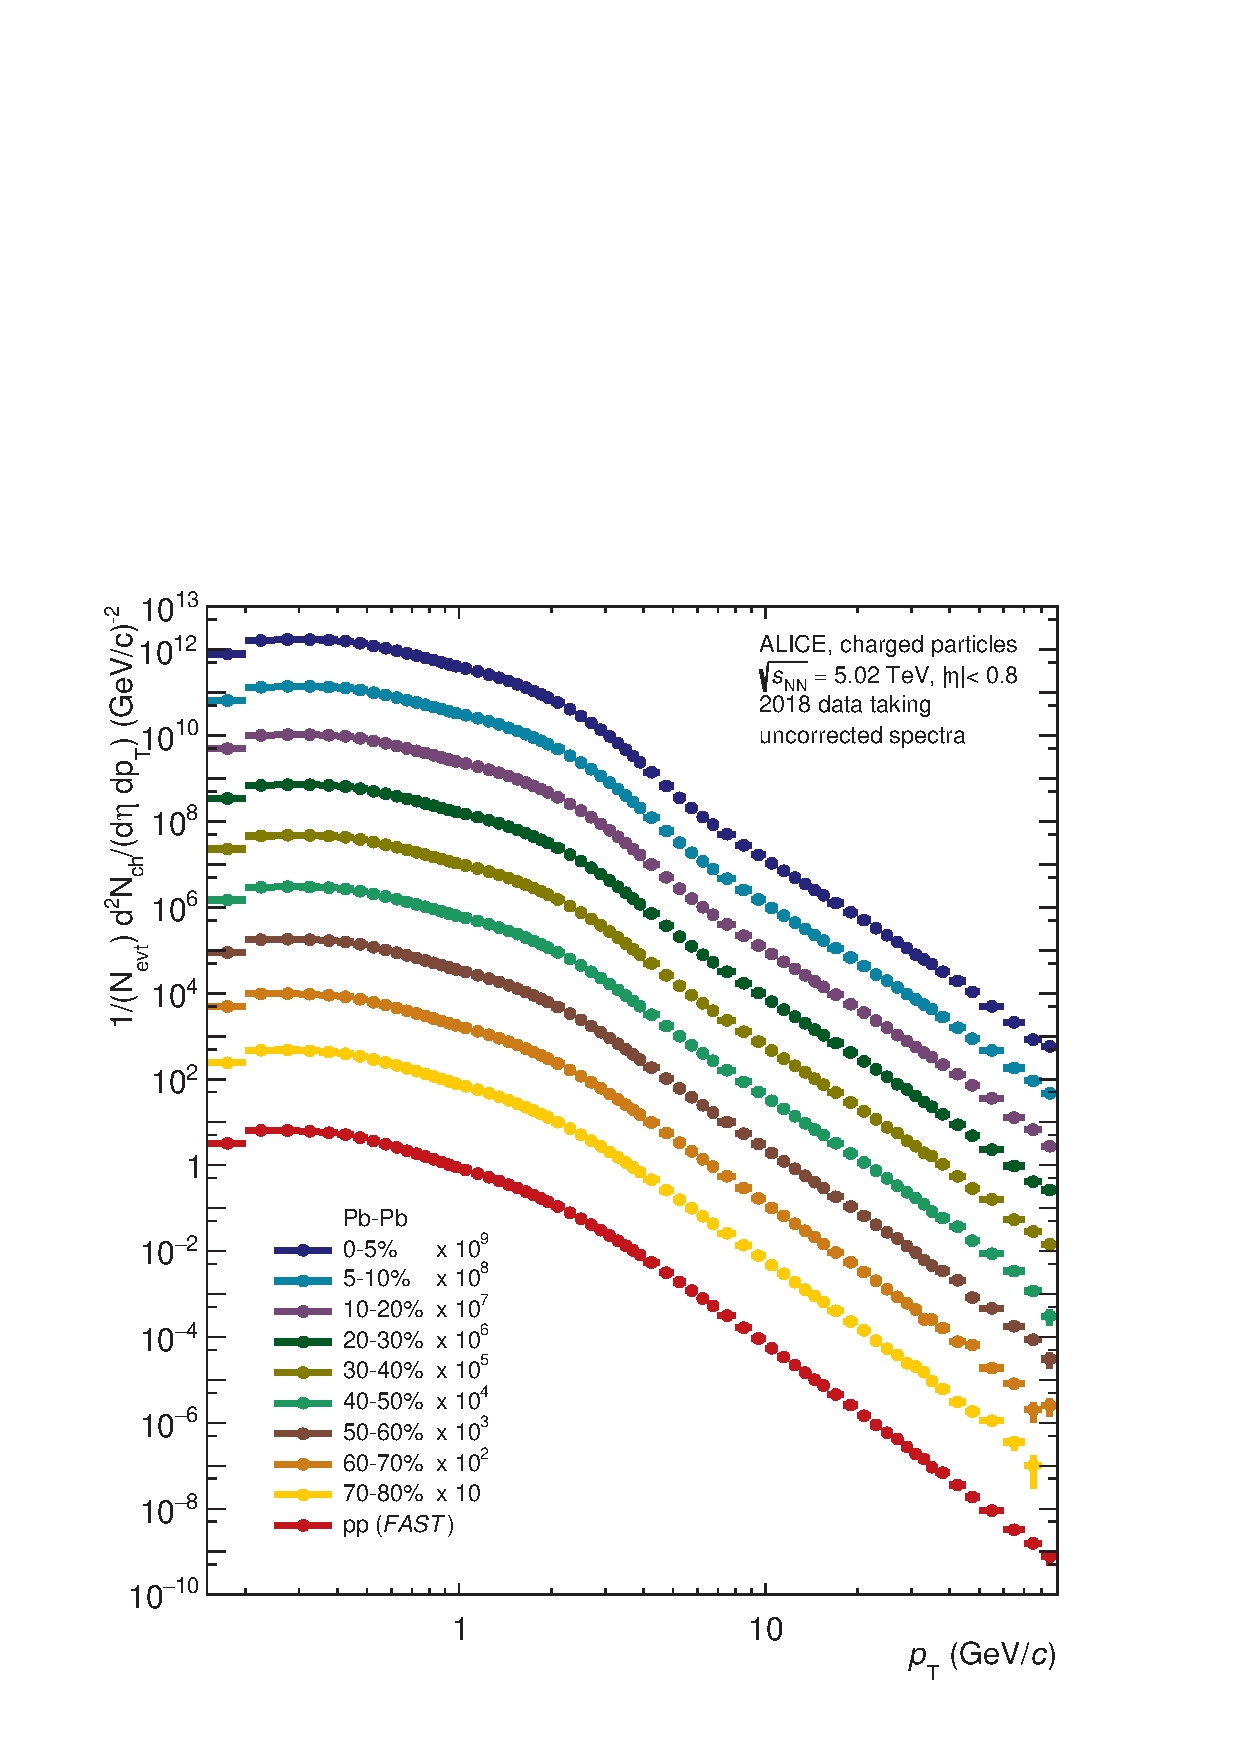
\includegraphics[width=0.45\textwidth]{Plots/uncorrectedSpectra.pdf} 
\caption{Uncorrected \pt spectra}
\end{figure}

\begin{itemize}
\item Uncorrected \pt spectra
\item Several detector effects must be corrected.
\item Track and event level corrections
\end{itemize}

\subsection{Normalisation of the pt spectrum}
\begin{itemize}
\item Follow line of argument presented in status update from 6.10.2020
\item Normalize with number of reconstruced events.
\item In case of pp, this number does not correspond number of inelastic events and must be therefore corrected (trigger and vertex efficiencies).
\item Trigger efficiency: ratio between visible and inelastic cross section. van-der-Meer scans were used for the determination of $\sigma_{vis}$, while sophisticated fit approximation for $\sigma_{inel}$. $\epsilon_{trig}$. Equal 1 in the case of Pb-Pb.
\item Vertex efficiency: ratio of the number of events with vertex to the number of triggered events. Equal 1 in the case of Pb-Pb.
\item Verex efficiency must be combined with a correction at track level in order to regain the signal loss.
\end{itemize}
\begin{figure}[tb!]
\centering
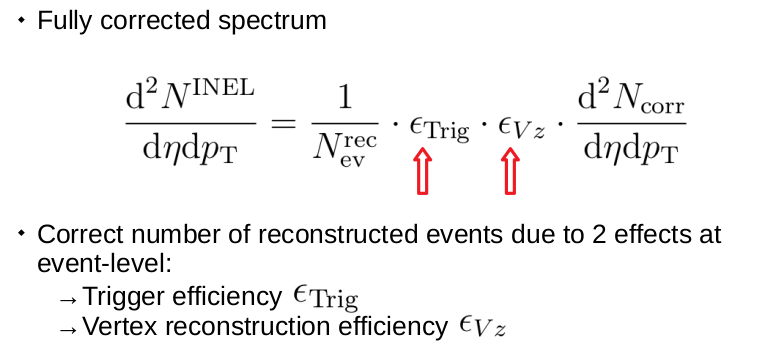
\includegraphics[width=0.45\textwidth]{Plots/DefinitionOfTheSpectrum.png} 
\caption{Normalisation of the pt spectrum} 
\end{figure}

\subsection{Tracking efficiency}
\begin{itemize}
\item Definition: reconstructed primary tracks/ generated  primary tracks. 
\item Describe shape: at low \pt efficiency increases due to the more sharper bending of the tracks in this \pt range. Then, efficiency decreases at \pt $= 1$ GeV  because of track length cut. 
\item In Pb-Pb: statistics are not sufficient large to divide tracking eff. in centrality classes (show plot). Instead scale the MB efficiency with a factor extracted from fitting the ratio cent. dependent eff to MB eff. (show plot). 
\item Particle compositon by Patrick. Yield of some strange particles is underestimated by MC generators. Therefore an additional correction is needed. Correction not implemented by presented analysis, but used. 
\end{itemize}
\begin{figure}[tb!]
\centering
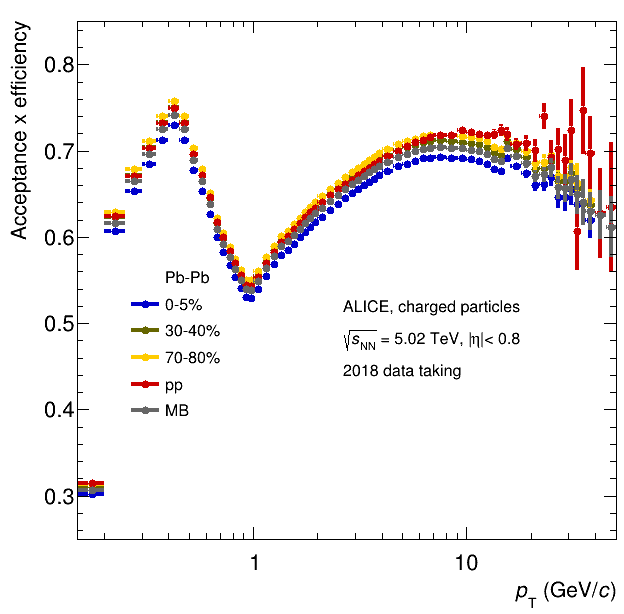
\includegraphics[width=9cm]{Plots/trckEff.png}  
\caption{Tracking efficiency} 
\end{figure}

\subsection{Secondary contamination}
\begin{itemize}
\item Even using track selection, a small amount of secondaries (decay products and particles esulting intereaction with detector material) remain. Use MC to correct this amount (show plot). 
\item More secondaries at low \pt, since secondaries take a fraction of the energy of the mother particle 
\item Again, the underestimation by the MC generators of strange particles (do research about this underestimation and describe it) must be corrected -> Secondary scaling.
\end{itemize}
\subsubsection{Secondary scaling} 
\begin{itemize}
\item Secondary scaling: make use of DCA disitributions, since those of primaries are different to those of secondaries. Use template fits (define template fit) using the MC predictions of the distributions to determine the fractions of secondaries in data (show DCA plot). Compare obtained fractions to MC fraction to calculate a \pt dependent correction factor. 
\item To get best possible results, \pt, multiplicity and DCA intervals were optimized.
\item To evaluate the quality of the fit, chi2-test and pulls were used (define chi2-test and pulls, show pull distributions).
\item Make plot with resulting correction factors. 
\end{itemize}
\begin{figure}[tb!]
\centering
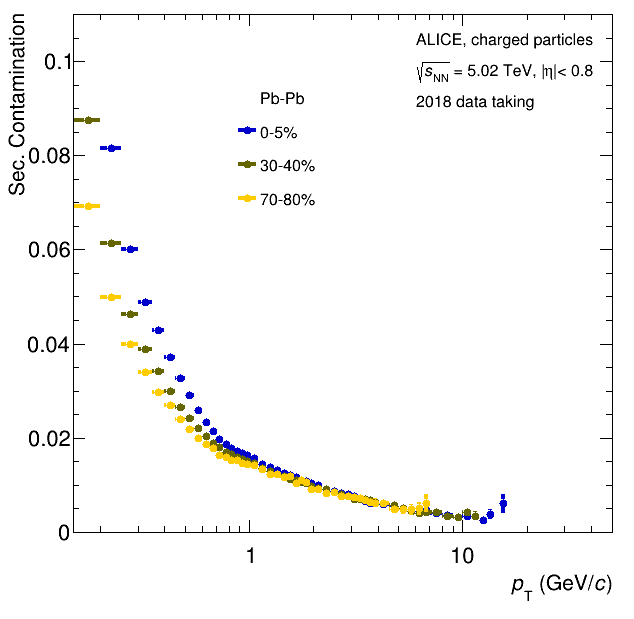
\includegraphics[width=9cm]{Plots/SecCont.png}  
\caption{Secondary Contamination} 
\end{figure}
\begin{figure}[tb!]
\centering
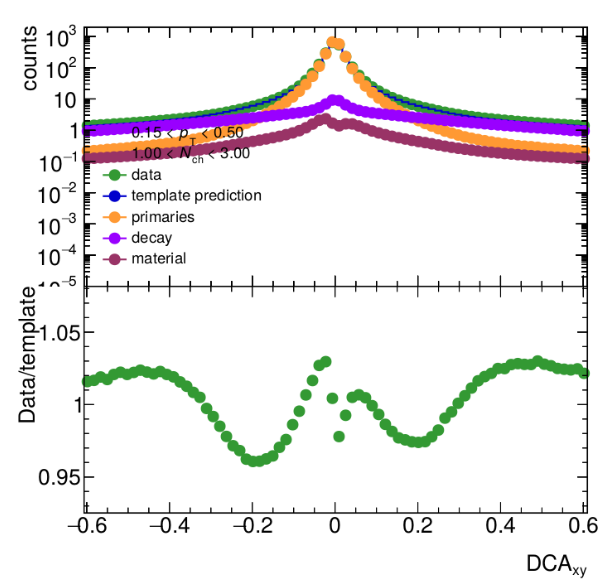
\includegraphics[width=9cm]{Plots/DCAdistribution.png}  
\caption{DCA distributions} 
\end{figure}
\subsection{\pt resolution correction}
Follor arguemnt line presentend on the status update from 7.4.2020
\begin{itemize}
\item Momentum determinaton explained in detector chapter. 1/\pt is a parameter of the covariance matrix, so we know its resolution. 
\item Gluckstern paper states $\sigma(p_\text{T})/p_\text{T} \approx p_\text{T}\sigma(1/p_\text{T})$
\item Present $\sigma(p_\text{T})/p_\text{T}$ distribution. At low \pt, it is dominated by multiple scattering. Minimum at 1 GeV/$c$. At high \pt, resolution increases because tracks get less curved
\item Due to the \pt resolution, the measured spectrum deviates from the true spectrum. This is expressed by means of a convolution between measured spectrum and function $R$ that characterize the detector response.
\item Correction factor needed. This is defined as ration of measured spectrum to convoluted measured spectrum.
\item Explain toy MC used to calculate the correction factor: Fit $<\sigma(1/p_\text{T})>$. Eliminate statistical fluctuations in $\sigma(1/p_\text{T})$  by extracting the fit from it. Project resulting  $\sigma(1/p_\text{T})$ along y axis. As result, one obtains the statsitical distribution of $\sigma(1/p_\text{T})$. Fit now the measured spectrum with a Hagedorn (this allows, of course, to get centrality dependent correction factors in the case of Pb-Pb col.). Use fit to produce a \pt distribution. Calculate 1/\pt and shift the distribution of  $\sigma(1/p_\text{T})$ so that the peak coincides with the corresponding $<\sigma(1/p_\text{T})>$ value. Genearate a $\sigma(1/p_\text{T})$ value randomly. Smear 1/\pt with this value assuming a gaussian form. Calculate \pt from smeared 1/\pt. Proudce a \pt distribution. Correction factor: ratio of measured spectrum to smeared measured spectrum. 
\end{itemize}
\begin{figure}[tb!]
\centering
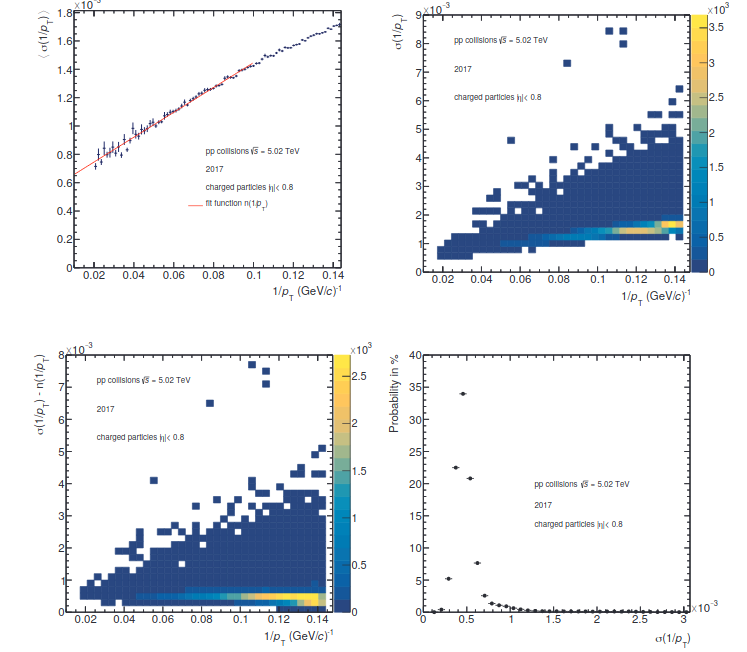
\includegraphics[width=9cm]{Plots/ptResolution.png}  
\caption{Method  used to obtain the statistical distribution of $\sigma(1/p_\text{T})$} 
\end{figure}
\begin{figure}[tb!]
\centering
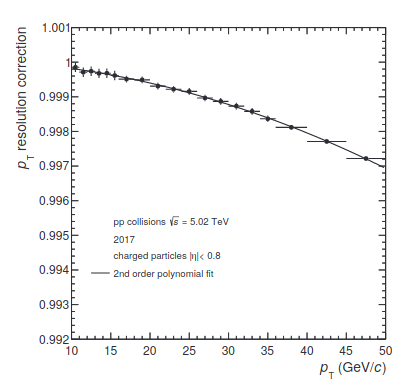
\includegraphics[width=9cm]{Plots/ptresolutionCorrFactor.png}
\caption{pt resolution correction factor} 
  
\end{figure}


\section{Corrected \pt spectra}
\begin{figure}[tb!]
\centering
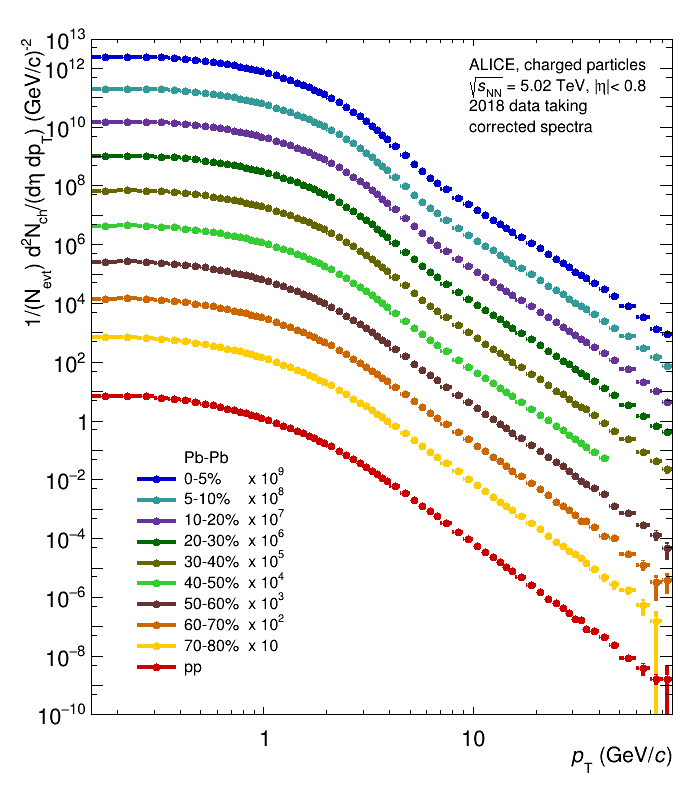
\includegraphics[width=9cm]{Plots/corrSpectra.png}  
\caption{Corrected \pt spectra}
\end{figure}
\begin{itemize}
\item In pp: Compare \pt spectra from CENT wSDD and CENT woSDD. If they match, combine FAST and CENT woSDD data sets.
\item In pp: Compare Edgar's fully corrected spectrum with mine. Emphazise the achivement of a more precise binning and a larger range.
\item In Pb-Pb: Compare Julius's fully corrected spectra with mine.
\end{itemize}

\section{Systematic uncertanties}
\begin{itemize}
\item Present systematic uncertanties of the spectra calculated performing cut variations. 
\end{itemize}
Calculate sys. uncertanties with method suggested by Joshua (calculate $R_\text{AA}$ for the different track cuts)
\section{Results}
Discuss $R_\text{AA}$ distributions including comparison with previous results.
\begin{figure}[tb!]
\centering
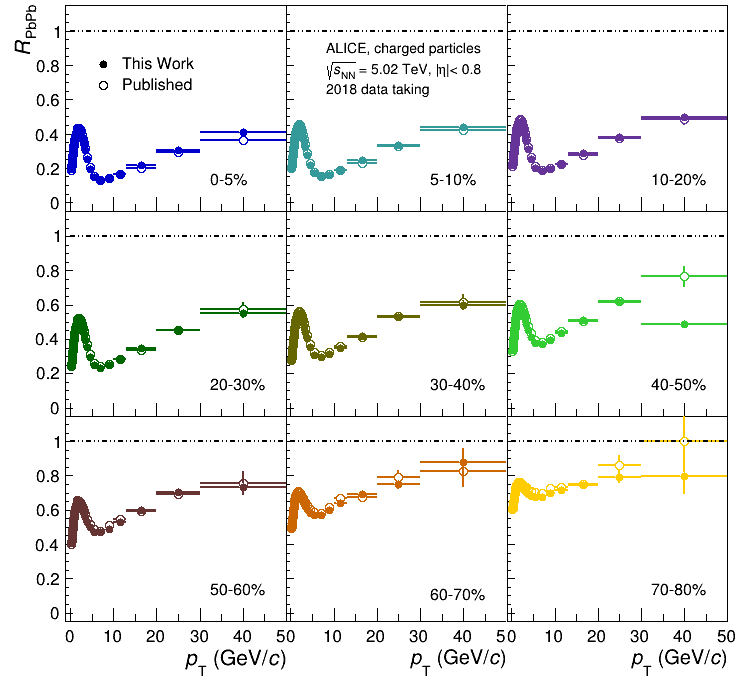
\includegraphics[width=9cm]{Plots/RaaRebinned.png} 
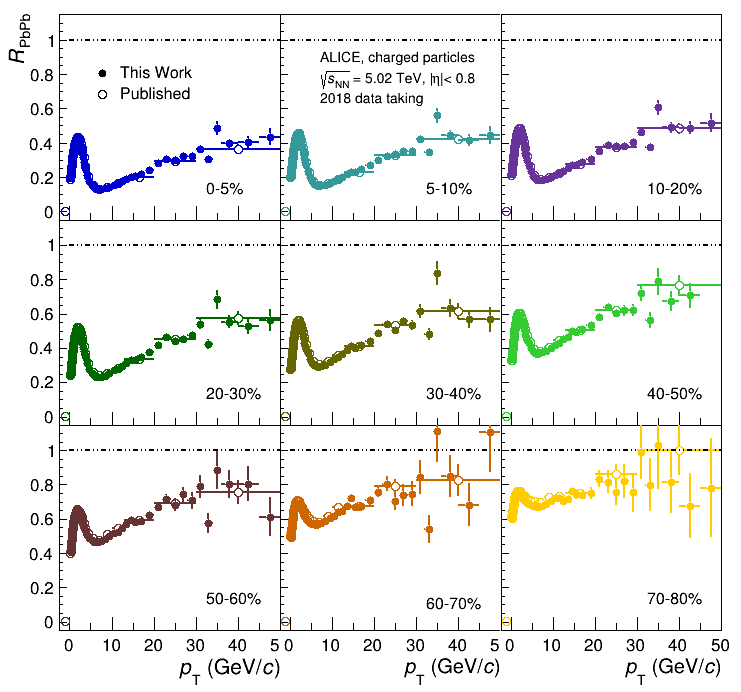
\includegraphics[width=9cm]{Plots/Raa.png} 
\caption{$R_\text{AA}$ (with and without rebin)}  
\end{figure}
\chapter{Summary}


%Moshi moshi Merle	
%Quellen: https://home.cern/science/physics/standard-model
%An Introduction to Particle Physics and the Standard Model by Robert Mann
%An Introduction to Particle Physics and the Standard Model of Particle Physics by Cottingham and Greenwood
%Physics Of The Standard Model And Beyond, The Chong-sa Lim, Toshiyuki Morii,

\end{document}
